\documentclass{article}

\newcommand{\bra}[1]{\left(#1\right)}
\usepackage[activate={true,nocompatibility},final,tracking=true,kerning=true,spacing=true,factor=1100,stretch=10,shrink=10]{microtype}
\microtypecontext{spacing=nonfrench}
\usepackage{tikz}
\usepackage{tikz-cd}
\usepackage{mathpazo}
\usepackage{amsmath,amsthm,amssymb}
\usepackage{subcaption}
\usepackage{enumerate}
\usetikzlibrary{shapes}
\usetikzlibrary{positioning}
% Set up the images/graphics package
\usepackage{graphicx,float}
\setkeys{Gin}{width=\linewidth,totalheight=\textheight,keepaspectratio}
\graphicspath{{.}}


% Small sections of multiple columns
\usepackage{multicol}
\usepackage[margin=1.6in]{geometry}

%--------Theorem Environments--------
%theoremstyle{plain} --- default
\newtheorem{thm}{Theorem}
\newtheorem{cor}[thm]{Corollary}
\newtheorem{prop}[thm]{Proposition}
\newtheorem{lem}[thm]{Lemma}
\newtheorem{conj}[thm]{Conjecture}
\newtheorem{quest}[thm]{Question}
\newtheorem{claim}{Claim}

\theoremstyle{definition}
\newtheorem{defn}[thm]{Definition}
\newtheorem{defns}[thm]{Definitions}
\newtheorem{con}[thm]{Construction}
\newtheorem{exmp}[thm]{Example}
\newtheorem{jk}[thm]{Joke}
\newtheorem{exmps}[thm]{Examples}
\newtheorem{notn}[thm]{Notation}
\newtheorem{notns}[thm]{Notations}
\newtheorem{addm}[thm]{Addendum}
\newtheorem{exer}[thm]{Exercise}

\theoremstyle{remark}
\newtheorem{rem}[thm]{Remark}
\newtheorem{ans}[thm]{Answer}
\newtheorem{rems}[thm]{Remarks}
\newtheorem{warn}[thm]{Warning}
\newtheorem{sch}[thm]{Scholium}

% MACROS
\newcommand{\Mod}[1]{\ (\text{mod}\ #1)}
\newcommand{\R}{\mathbb{R}}
\newcommand{\N}{\mathbb{N}}
\newcommand{\Q}{\mathbb{Q}}
\newcommand{\F}{\mathbb{F}}
\newcommand{\Z}{\mathbb{Z}}
\newcommand{\mC}{\mathcal{C}}
\newcommand{\mG}{\mathcal{G}}
\newcommand{\mP}{\mathcal{P}}
\newcommand{\one}{\mathbb{1}}
\renewcommand{\P}{\mathbb{P}}
\DeclareMathOperator{\dist}{dist}
\DeclareMathOperator{\aut}{Aut}
\DeclareMathOperator{\gal}{Gal}
\DeclareMathOperator{\orb}{Orb}
\DeclareMathOperator{\stab}{Stab}
\DeclareMathOperator{\inn}{Inn}
\DeclareMathOperator{\spn}{Span}
\DeclareMathOperator{\out}{Out}
\DeclareMathOperator{\im}{Im}
\DeclareMathOperator{\arr}{Arr}
\DeclareMathOperator{\rk}{rk}
\DeclareMathOperator{\rcf}{rcf}
\DeclareMathOperator{\tors}{Tors}
\DeclareMathOperator{\Hom}{Hom}
\DeclareMathOperator{\ann}{Ann}
\DeclareMathOperator{\syl}{Syl}
\newcommand{\norm}[1]{\left\lVert #1 \right\rVert}
\newcommand{\inp}[2]{\left\langle #1, #2 \right\rangle}
\newcommand{\id}{\text{id}}
\newcommand{\gln}{\text{GL}_n}
\newcommand{\op}[1]{#1^{\text{op}}}

\title{Lecture 1 - Categories and Functors\vspace{-10pt}}
\author{Ralph Sarkis}
\date{\vspace{-10pt}May 8, 2019\vspace{-20pt}}  % if the \date{} command is left out, the current date will be used
\begin{document}
\maketitle
\begin{abstract} Categories and functors will be introduced as well as lots of examples coming from diverse subfields of mathematics.
\end{abstract}
\setcounter{section}{-1}
\section{Introduction}
This is the first lecture of a series exploring the basic concepts in category theory. The aim is to teach undergraduate students about these topics by considering their application in various subfields of mathematics as well as the theory on its own. The in-person lectures will only assume knowledge of U1 courses in mathematics, such as abstract algebra, analysis and basics of set theory (what is usually taught in the aforementioned classes). New objects will be defined during the lectures but if you are reading these notes without attending the lectures, you may have to look up definitions online.

Before diving into this topic, we discuss the necessary distinction between sets and classes. Several times in our coverage of category theory, we will need to use the concept of a class. It is very similar to that of a set and has one simple difference. While a set \textit{can} contain another set, classes \textit{cannot} contain other classes.

This difference is indispensable because some collections of objects can simply not form a set. Famous examples include the class of ordinal numbers which, by the Burali-Forti paradox, cannot be a set and the class of all sets that do not contain themselves which, by the Russel paradox, cannot be a set. In addition, we will soon talk about the class of all sets and the class of all groups (among others) and these classes are \textbf{proper}, that is, they are not sets. For the former, it is easy to see because if $S$ is the set of all sets, then it contains all its subsets and hence $\mP(S) \subseteq S$, this leads to the contradiction $|\mP(S)| \leq |S| < |\mP(S)|$.

Fortunately, these lectures will not require a profound understanding of this distinction as we will essentially use classes as if they were sets. Thus, to avoid confusion, one could replace the word ``class`` with ``collection`` and still follow the theory we present.
\section{Categories}
\begin{defn}[Oriented graph]
	An \textbf{oriented graph} $G$ consists of a class of \textbf{nodes/objects} denoted $G_0$ and a class of \textbf{arrows/morphisms} denoted $G_1$ along with two maps $s,t: G_1 \rightarrow G_0$, so that each arrow $f \in G_1$ has a \textbf{source} $s(f)$ and a \textbf{target} $t(f)$. 
\end{defn}
\begin{defn}[Paths]
	A \textbf{path} in an oriented graph $G$ is a sequence of arrows $(f_1, \dots, f_k)$ that are \textbf{composable} in the sense that $t(f_i) = s(f_{i-1})$ for $i=2,\dots, k$ as seen below. The class of paths of length $k$ will be denoted $G_k$.
	\begin{figure}[h!]
		\centering
		\begin{tikzcd}
			\bullet \arrow[r, "f_k"] & \bullet \arrow[r, "f_{k-1}"] & \bullet\cdots\bullet \arrow[r, "f_2"] & \bullet \arrow[r, "f_1"] & \bullet
		\end{tikzcd}
		\caption*{Representation of path $(f_1, \dots, f_k)$.}
	\end{figure}
\end{defn}
Observe that the notation indicating the direction of the path does not correspond to the usual notation in graph theory. The motivation for this divergence will come shortly as the composition of arrows in a category is defined, the main idea is that the morphisms will correspond to functions between mathematical objects rather than arrows between nodes of a graph.
\begin{defn}[Category]
	An oriented graph $C$ along with a composition map $\circ: C_2 \rightarrow C_1$ is a \textbf{category} if it satisfies the following properties.
	\begin{enumerate}
		\item For any $(f, g) \in C_2$, $s(f \circ g) = s(g)$ and $t(f \circ g) = t(f)$. This is more naturally understood in the diagram below.
		\begin{figure}[h]
			\centering
			\begin{tikzcd}
				\bullet \arrow[r, "g"'] \arrow[rr, "f \circ g", bend left] & \bullet \arrow[r, "f"'] & \bullet
			\end{tikzcd}
		\end{figure}
		\item For any $(f,g,h) \in C_3$, $f\circ(g\circ h) = (f\circ g)\circ h$, namely, composition is associative.
		\item For any $A \in C_0$, there exists an \textbf{identity} morphism $u_C(A) \in C_1$ with $A$ as its source and target that satisfies $u_C(A) \circ f = f$ and $g \circ u_C(A) = g$, for any $f,g \in C_1$ where $t(f) = A$ and $s(g) = A$.
	\end{enumerate}
\end{defn}
\begin{rem}[Notation]
	In general, we will denote categories with $C$ or $D$, their objects with uppercase letters ($A$, $B$, $X$, $Y$, $Z$, etc.) and their morphisms with lowercase letters ($f$, $g$, $h$, etc.). When the category is clear from the context, we denote the identity morphism $\id_A$ instead of $u_C(A)$.
\end{rem}
If the third property is not satisfied, $C$ is referred to as a \textbf{semicategory}. Some authors choose to explicit when a category \textit{does} satisfy the second property, qualifying it as \textbf{unital}, but this term also has other meanings, hence our preference for the first convention.

Moreover, since $\circ$ is associative, it induces a unique composition map on paths of any finite lengths. This lets us write $f_1 \circ f_2 \circ \cdots \circ f_k$ with no parentheses as well as abuse notation and write $\circ: C_k \rightarrow C_1$. Occasionally, we will mention the composition of a path to mean the image of the path under this map.
\begin{exmps}[Boring examples]
	It is really easy to construct a category by drawing the oriented graph and inferring the definition of the composition from it. For instance, diagram (a) below corresponds to the category with objects $\{A, B\}$ and morphisms $\{\id_A, \id_B, f\}$. The composition map is then completely determined by the properties of identity morphisms.
	\begin{figure}[h]
		\centering
		\minipage[b]{.3\textwidth}
			\centering
			\begin{tikzcd}
				\bullet \arrow[r, "f"] & \bullet
			\end{tikzcd}
			\caption*{(a) Simple example.}
		\endminipage
		\minipage[b]{.3\textwidth}
			\centering
			\begin{tikzcd}
				\bullet \arrow[r] \arrow[d] \arrow[rd, bend left] \arrow[rd, bend right] & \bullet \arrow[d] \\
				\bullet \arrow[r]                                                        & \bullet          
			\end{tikzcd}
			\caption*{(b) Ambiguous square.}
		\endminipage
		\minipage[b]{.3\textwidth}
			\centering
			\begin{tikzcd}
				\bullet \arrow[r] \arrow[d] & \bullet \arrow[d] \\
				\bullet \arrow[r]           & \bullet          
			\end{tikzcd}
			\caption*{(c) Commutative square.}
		\endminipage
	\end{figure}

	The identity morphisms are omitted from the diagrams for clarity reasons (i.e.: they would hinder readability without adding information). However, if two distinct morphisms have the same source and target, they must be explicitly drawn and the ambiguity in the composition must be removed. For instance, diagram (b) has two distinct paths of length two starting at the top-left corner and ending at the bottom-right corner. Since the composition of the bottom left path can correspond to any of the two distinct morphisms between these corners, and similarly for the top right path, the category is ambiguous.
	
	Diagram (c) shows a very important example of a simple category that handles this problem. It is implicitly stating that the bottom and top path compose to the same morphism, the latter is thus absent of the diagram. The term ``commutative`` can also be generalized to larger diagrams, it means that for any two objects connected by a directed path, there is a unique arrow connecting the two objects. In other words, if two paths have the same source and target, then the compositions of both paths yield the same arrow.
\end{exmps}
Before moving on to more interesting examples, we mention a notation that we will frequently use.
\begin{defn}
	Let $C$ be a category and $A,B \in C_0$ be objects, the collection of all morphisms going from $A$ to $B$ is 
	\[\Hom_{C}(A,B) = \{f \in C_1 \mid s(f) = A \text{ and } t(f) = B\}.\]
	This leads to an alternative way of defining the morphisms of $C$, namely, one can describe $\Hom_C(A,B)$ for all $A, B \in C_0$ instead of describing all of $C_1$ at once. 
\end{defn}
\begin{defn}[Smallness]
	A category $C$ is called \textbf{small} if the classes of objects and morphisms are not proper, that is, they are sets. If for all objects $A,B \in C_0$, $\Hom_C(A,B)$ is a set, $C$ is said to be \textbf{locally small} and $\Hom_C(A,B)$ is called a \textbf{Hom-set}.
\end{defn}
\begin{exmp}[\textbf{\textbf{Set}}]
	The category \textbf{Set} has the class of sets as its objects and for any sets $X$ and $Y$, $\Hom_{\textbf{Set}}(X,Y)$ contains all the functions from $X$ to $Y$. The composition map is the usual one, the associativity follows from the definition and the identity maps serve as the identity morphisms. This category is locally small but not small.
\end{exmp}
\begin{exmp}
	Let $(X, \leq)$ be a partially ordered set, then $X$ can be viewed as a category with elements of $X$ as its objects. For any $x,y \in X$, the Hom-set $\Hom_X(x,y)$ contains a single morphism if $x \leq y$ and is empty otherwise. Since every Hom-set contains at most one element and $\leq$ is transitive, the composition map is completely determined and well-defined. The identity morphisms arise from the reflexivity of $\leq$.
	
	Let $(X, \tau)$ be a topological space, note that the inclusion of open sets is a partial order on $\tau$, thus $X$ has a corresponding category as above. More explicitly, the objects are open sets and for any $U, V \in \tau$, the Hom-set $\Hom_X(U,V)$ contains the inclusion map $i_{UV}$ if $U\subseteq V$ and is empty otherwise.
	\begin{figure}[h]
		\centering
		\begin{tikzcd}
			\stackrel{0}{\bullet} \arrow[r] & \stackrel{1}{\bullet} \arrow[r] & \stackrel{2}{\bullet} \arrow[r] & \cdots
		\end{tikzcd}
		\caption*{Category associated to the natural numbers $(\N, \leq)$.}
	\end{figure}
\end{exmp}
\begin{exmp}[Single object categories]
	If a category $C$ has a single object $\ast$, then the only morphisms go from $\ast$ to $\ast$. In particular, $C_1 = \Hom_C(\ast, \ast)$ and $C_2 = C_1 \times C_1$. Then, the associativity of $\circ$ and existence of $\id_{\ast}$ makes $(C_1, \circ)$ into a monoid.
	
	Conversely, a monoid $(M, \cdot)$ can be represented by a single object category $M$, where $\Hom_M(\ast, \ast) = M$ and the composition map is the monoid operation.
	
	Since many algebraic structures have a an associative operation and an identity element, this yields a fairly general construction. If such a structure is denoted $X$, then we will denote its associated category by $X\ast$.
		\begin{figure}[h]
		\begin{center}
			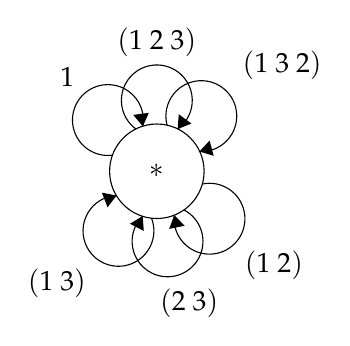
\begin{tikzpicture}[scale=0.2]
			\tikzstyle{every node}+=[inner sep=0pt]
			\draw [black] (37.4,-25.7) circle (3);
			\draw (37.4,-25.7) node {$\ast$};
			\draw [black] (34.593,-24.676) arc (277.6886:-10.3114:2.25);
			\draw (31.72,-20.34) node [above] {$1$};
			\fill [black] (36.51,-22.85) -- (36.89,-21.99) -- (35.9,-22.12);
			\draw [black] (40.276,-26.512) arc (101.97044:-186.02956:2.25);
			\draw (42.95,-31.68) node [right] {$(1\ 2)$};
			\fill [black] (38.51,-28.48) -- (38.18,-29.36) -- (39.16,-29.16);
			\draw [black] (39.111,-28.15) arc (62.6723:-225.3277:2.25);
			\draw (39.45,-33.13) node [below] {$(2\ 3)$};
			\fill [black] (36.5,-28.55) -- (35.69,-29.03) -- (36.57,-29.49);
			\draw [black] (37.059,-28.669) arc (21.17668:-266.82332:2.25);
			\draw (31.05,-31.87) node [below] {$(1\ 3)$};
			\fill [black] (34.84,-27.24) -- (33.91,-27.06) -- (34.27,-27.99);
			\draw [black] (36.077,-23.02) arc (234:-54:2.25);
			\draw (37.4,-18.45) node [above] {$(1\ 2\ 3)$};
			\fill [black] (38.72,-23.02) -- (39.6,-22.67) -- (38.79,-22.08);
			\draw [black] (38.053,-22.784) arc (195.11223:-92.88777:2.25);
			\draw (45.36,-19.95) node [above] {$(1\ 3\ 2)$};
			\fill [black] (40.11,-24.44) -- (41.01,-24.72) -- (40.75,-23.75);
			\end{tikzpicture}
		\end{center}
		\caption*{Category corresponding to the symmetric group $S_3$.}
	\end{figure}
\end{exmp}
A lot of simple examples of ``large`` categories arise as subcategories of \textbf{Set}.
\begin{defn}[Subcategory]
	Let $C$ be a category, a category $C'$ is a \textbf{subcategory} of $C$ if, the following intuitive properties are satisfied.
	\begin{enumerate}
		\item The objects and morphisms of $C'$ are objects and morphisms of $C$ (i.e.: $C'_0 \subseteq C_0$ and $C'_1 \subseteq C_1$).
		\item The source and target maps of $C'$ are the restrictions of the source and target maps of $C$ on $C'_1$ and for every morphism $f \in C'_1$, $s(f), t(f) \in C'_0$.
		\item The composition map of $C'$ is the restriction of the composition map of $C$ on $C'_2$ and for any $(f,g) \in C'_2$, $f\circ_{C'} g = f \circ_{C} g \in C'_1$. 
	\end{enumerate}
	A formal consequence of 3 is that the identity morphisms of objects in $C'_0$ are the same whether they are seen in $C$ or $C'$.
\end{defn}
\begin{defn}[Full and wide]
	A subcategory $C'$ of $C$ is called \textbf{full} if for any objects $A,B \in C'_0$, $\Hom_{C'}(A,B) = \Hom_{C}(A,B)$. It is called \textbf{wide} if $C'_0 = C_0$.
\end{defn}
\begin{exmps}[Subcategories of \textbf{Set}]
	One can view most of the theory studied in the first year of a typical mathematics curriculum through the lens of category theory as witnessed by the following list.
	\begin{enumerate}
		\item Since the composition of injective functions is again injective, the restriction of morphisms to injective functions yields a wide subcategory of \textbf{Set}, denoted \textbf{SetsInj}. Unsurprisingly, \textbf{SetsSurj} can be constructed similarly.
		\item The full subcategory of finite sets is denoted \textbf{FinSet}.
		\item The category of groups (resp\,rings or fields) where the morphisms are group (resp\,ring or field) homomorphisms is denoted \textbf{Grp}/\textbf{Ring}/\textbf{Field}.
		\item Let $k$ be a fixed field, the category of vector spaces over $k$ where the morphisms are linear maps is denoted $\textbf{Vsp}_k$.
		\item The category of partially ordered sets where morphisms are order-preserving functions is denoted \textbf{Poset}.
		\item The category of topological spaces where morphisms are continuous functions is denoted \textbf{Top}.
	\end{enumerate}
\end{exmps}

\section{Functors}
The above list is far from being exhaustive; there are many more mathematical objects that can fit in a category and this is a main reason for studying this subject. Indeed, categories encapsulate a natural structure that accurately represents the heart of several mathematical theories from a global and abstract perspective. Still, a category is almost never studied on its own and we will probably see in later lectures that some surprising links can arise between seemingly unrelated subjects (e.g.: Stone duality). The central tool for exhibiting these relations is a functor.
\begin{defn}[Functor]
	Let $C$ and $D$ be categories, a \textbf{functor} $F: C \rightsquigarrow D$ is a pair of maps $F_0:C_0 \rightarrow D_0$ and $F_1:C_1 \rightarrow D_1$ such that the following diagrams commute (where $F_2$ is induced by the definition of $F_1$ with $(f,g) \mapsto (F_1(f), F_1(g))$).
	\begin{figure}[h]
		\centering
		\begin{tikzcd}
			C_0 \arrow[d, "F_0"'] & C_1 \arrow[d, "F_1"] \arrow[l, "s"'] \arrow[r, "t"] & C_0 \arrow[d, "F_0"] \\
			D_0 & D_1 \arrow[l, "s"] \arrow[r, "t"'] & D_0
		\end{tikzcd}
		\qquad 
		\begin{tikzcd}
			C_2 \arrow[d, "\circ_C"'] \arrow[r, "F_2"] & D_2 \arrow[d, "\circ_D"] \\
			C_1 \arrow[r, "F_1"'] & D_1
		\end{tikzcd}
		\qquad
		\begin{tikzcd}
			C_0 \arrow[d, "u_C"'] \arrow[r, "F_0"] & D_0 \arrow[d, "u_D"] \\
			C_1 \arrow[r, "F_1"'] & D_1
		\end{tikzcd}
	\end{figure}
\end{defn}
\begin{rem}[Digesting diagrams]
	Commutative diagrams will be heavily employed to make clearer and more compact arguments (especially on the board). However, it is an acquired skill to quickly grasp their meaning and make effective use of their advantages. Unpacking the above definition will help to understand it as well as getting better with manipulating diagrams.
	
	A functor $F:C\rightsquigarrow D$ must satisfy the following properties.
	\begin{enumerate}[i.]
		\item For any $A, B \in C_0$, if $f \in \Hom_C(A,B)$ then $F(f) \in \Hom_D(F(A), F(B))$.
		\item If $f,g \in C_1$ are composable, then $F(f\circ g) = F(f) \circ F(g)$.
		\item If $A \in C_0$, then $u_D(F(A)) = F(u_C(A))$.
	\end{enumerate}
	The subscript on $F$ is omitted, as is common in the literature, because it is always clear whether $F$ is applied to an object or a morphism.
\end{rem}
\begin{exmps}[Boring examples]
	As is usual, a few trivial constructions arise.
	\begin{enumerate}
		\item For any category $C$, the identity functor $\one: C\rightsquigarrow C$ is defined by letting $\one_0$ and $\one_1$ be identity maps on $C_0$ and $C_1$ respectively.
		\item Let $C$ be a category and $C'$ a subcategory of $C$, the inclusion functor $I: C' \rightsquigarrow C$ is defined by letting $I_0$ be the inclusion map $C'_0 \hookrightarrow C_0$ and $I_1$ be the inclusion map $C'_1 \hookrightarrow C_1$.
		\item Let $C$ and $D$ be categories and $X$ be an object in $D$, the constant functor $X: C \rightsquigarrow D$ is defined by letting $X(A) = X$ for any $A \in C_0$ and $X(f) = \id_X$ for any $f \in C_1$.
	\end{enumerate}
\end{exmps}
Throughout these lectures, the goal will be essentially to grow this list with more and more interesting functors and perhaps exploit their behavior wisely. Before pursuing this objective, we give important definitions analogous to injectivity and surjectivity of functions.
\begin{defn}[Full and faithful]
	Let $F:C \rightsquigarrow D$ be a functor. For $A,B \in C_0$, denote the restriction of $F_1$ to $\Hom_C(A,B)$ with \[F_{A,B}:\Hom_C(A,B) \rightarrow \Hom_D(F(A), F(B)).\]
	\begin{itemize}
		\item If $F_{A,B}$ is injective for any $A,B \in C_0$, then $F$ is \textbf{faithful}.
		\item If $F_{A,B}$ is surjective for any $A,B \in C_0$, then $F$ is \textbf{full}.
		\item If $F_{A,B}$ is bijective for any $A,B \in C_0$, then $F$ is \textbf{fully faithful}.
	\end{itemize}    
\end{defn}
\begin{exmps}
	\begin{enumerate}
		\item[]
		\item The power set functor $\mP: \textbf{Set} \rightsquigarrow \textbf{Set}$ sends a set $X$ to its power set $\mP(X)$ and a function $f: X\rightarrow Y$ to the image map $\mP(f):\mP(X)\rightarrow \mP(Y)$, the latter sends a subset $S\subseteq X$ to \[f(S) = \{f(s) \mid s \in S\} \subseteq Y.\]
		The power set functor is faithful because the same image map cannot arise from two different functions, it is not full because lots of functions $\mP(X) \rightarrow \mP(Y)$ are not image maps. One can also argue by cardinality because (when $|X|, |Y| \geq 2$)
		\[|\Hom_{\textbf{Set}}(X,Y)| = |Y|^{|X|} < |\mP(Y)|^{|\mP(X)|} = |\Hom_{\textbf{Set}}(\mP(X), \mP(Y))|.\]
		\item While in general the inclusion functor of a subcategory is not interesting, there are some distinguished cases. For instance, when considering subcategories of \textbf{Set} such as those mentioned earlier, this functor gets a fancier denomination, namely, the \textbf{forgetful} functor. This is because, morally, the functor is forgetting about the inner structure of the objects and morphisms and it outputs the underlying sets and functions.
		
		\item It is also sometimes useful to consider "intermediate" forgetful functors. For instance, $\Phi: \textbf{Ring} \rightsquigarrow \textbf{AbGrp}$ sends a ring $(R, +, \cdot)$ to the abelian group $(R, +)$. It does not need to affect morphisms because part of the requirements for ring homomorphisms is to preserve the underlying additive group structure.
		
		\item In some cases, there is a non-trivial way to go in the opposite direction of the forgetful functor, that is, the \textbf{free} functor. For \textbf{Grp}, the free functor $F: \textbf{Set} \rightsquigarrow \textbf{Grp}$ sends a set to the free group generated by this set and a function $f: X\rightarrow Y$ to the unique group homomorphism $F(X) \rightarrow F(Y)$ that restricts to $f$ on the set of generators.
		
		Later in the notes, when covering adjunctions, we will study a strong relation between the forgetful functor $\Phi: \textbf{Grp} \rightsquigarrow \textbf{Set}$ and $F$ that will generalize to other algebraic structures.
		
		\item Let $(X, \leq)$ and $(Y, \subseteq)$ be posets, and $F:X\rightsquigarrow Y$ be a functor. For any $a, b \in X$, if $a\leq b$, then $\Hom_X(a,b)$ contains a single element, thus $\Hom_Y(F(a), F(b))$ must contain a morphism as well, or equivalently $F(a) \subseteq F(b)$. In other words, $F$ is an order-preserving function on the objects.
		
		Conversely, any order-preserving functions between $X$ and $Y$ will correspond to a unique functor since there is only one morphism in all the Hom-sets.
				
		\item Let $G$ and $H$ be groups and $G\ast$ and $H\ast$ be the single object categories they are associated to, then the functors $F: G\ast \rightsquigarrow H\ast$ are exactly the group homomorphisms from $G$ to $H$.
		
		\item For any group $G$, the functors $F:G\ast \rightsquigarrow \textbf{Set}$ are in correspondence with group actions of $G$. Indeed, if $S = F(\ast)$, then \[F_1: G = \Hom_{G\ast}(\ast, \ast) \rightarrow \Hom_{\textbf{Set}}(S, S)\]
		is such that $F(gh) = F(g) \circ F(h)$ for any $g,h \in G$ and $F(1) = \id_S$. Moreover, since for any $g \in G$,
		\[\id_S = F(1) = F(gg^{-1}) = F(g) \circ F(g^{-1}),\]
		the function $F(g)$ is a bijection and we conclude $F_1$ is the permutation representation of the group action.
	\end{enumerate}
\end{exmps}
%Functoriality is useful to prove stuff. If you know about the fundamental group. One can show brouwer fixed point theorem using this.
A clear similarity between categories like \textbf{Set}, \textbf{Grp}, \textbf{Ring} or \textbf{Top} is that all the objects have a minimum of structure that the morphisms preserve. In this lecture, we introduced a novel structure, namely categories, that functors preserve. Hence it is reasonable to wonder if categories are also part of a category. In fact, the only missing ingredient is the composition of functors (we already know what the source and target of a functor is and every category has an identity functor). After proving the following proposition, we end up with the category \textbf{Cat} where objects are categories and morphisms are functors. In order to avoid paradoxes of the Russel kind, it is essential to restrict \textbf{Cat} to contain only small categories.
\begin{prop}
	Let $F:C\rightsquigarrow D$ and $G: D\rightsquigarrow E$ be functors and $G \circ F:C \rightsquigarrow E$ be their composition defined (naturally) by $G_0 \circ F_0$ on objects and $G_1 \circ F_1$ on morphisms. Then, $G \circ F$ is a functor.
\end{prop}
\begin{proof}
	One could proceed with a really hands-on proof and show that $G \circ F$ satisfies the three necessary properties in a straightforward manner. While this should not be too hard, the proof will end up involving objects, morphisms and the composition from all three different categories. This can easily lead to confusion or worse, boredom.
	
	Instead, we will use the diagrams we introduced in the first definition of a functor. From the functoriality of $F$ and $G$, we get two sets of three diagrams and combining them yields the diagrams for $G \circ F$.
	
	\begin{figure}[h!]
		\centering
		\begin{tikzcd}
			C_0 \arrow[d, "F_0"'] & C_1 \arrow[d, "F_1"] \arrow[r, "t"] \arrow[l, "s"'] & C_0 \arrow[d, "F_0"] \\
			D_0 \arrow[d, "G_0"'] & D_1 \arrow[d, "G_1"] \arrow[r, "t"] \arrow[l, "s"'] & D_0 \arrow[d, "G_0"] \\
			E_0                   & E_1 \arrow[r, "t"] \arrow[l, "s"']                  & E_0                 
		\end{tikzcd}
		\quad
		\begin{tikzcd}
			C_2 \arrow[r, "F_2"] \arrow[d, "\circ_C"'] & D_2 \arrow[r, "G_2"] \arrow[d, "\circ_D"] & E_2 \arrow[d, "\circ_E"] \\
			C_1 \arrow[r, "F_1"']                      & D_1 \arrow[r, "G_1"']                     & E_1                     
		\end{tikzcd}
		\quad
		\begin{tikzcd}
			C_0 \arrow[r, "F_0"] \arrow[d, "u_C"'] & D_0 \arrow[r, "G_0"] \arrow[d, "u_D"] & E_0 \arrow[d, "u_E"] \\
			C_1 \arrow[r, "F_1"']                  & D_1 \arrow[r, "G_1"']                 & E_1                 
		\end{tikzcd}
	\end{figure}

	Almost no argument is needed here as the commutativity of the smaller diagrams clearly implies the commutativity of the combined diagrams. One information that is not shown above is the fact that $(G\circ F)_2 = G_2 \circ F_2$, but it would be pedantic to prove this.
\end{proof}
Since functors are also a new structure, one might expect that there are transformations between functors that preserve it. It is indeed the case as we will see later when presenting natural transformations. Moreover, although we might not cover it, there is a whole tower of abstraction that one could build in this way and it is the subject of study of higher category theory.

\section{Exercises (very optional)}
\begin{enumerate}
	\item Come up with your own ``interesting`` category. (Do not draw a simple diagram, look for examples from your previous classes.)
	\item Among the functors that were mentioned above, which ones are full? faithful?
	\item Pick your favorite functor that was mentioned and rigorously show that it is a functor.
	\item Convince yourself or prove rigorously that combining two commutative diagrams yields a commutative diagram.
	\item Show the last proposition following the sketch in the first paragraph of the proof.
\end{enumerate}
%Talk about more basic stuff in the theory of category in first part and in second part. go one level of abstraction higher to nat transformation and add more examples.
\end{document}

